%!TEX root = ../hycas2010.tex
%%%%%%%%%%%%%%%%%%%%%%%%%%%%%%%%%%%%%%%%%%%%%%%%%%%%
\section{A Case Example: The Hanoi Towers Robot}\label{sec:hanoi}
%%%%%%%%%%%%%%%%%%%%%%%%%%%%%%%%%%%%%%%%%%%%%%%%%%%%

\newcommand{\entity}[1]{\texttt{#1}}

To evaluate our learning framework we consider an existing BDI program
from the \JACK\ agent platform
distribution~\cite{BusettaRHL:AL99-JACK}.
% %
The example involves a robot playing the well-known Towers of Hanoi game where the goal is to stack discs of decreasing size onto a single pin. The rules of the game forbid discs to be moved onto smaller discs, however top discs may be moved onto discs of larger size across three pins. The problem is interesting for our purposes since the example solution makes use of parameterised event-goals and recursion. Furthermore, unlike our previous evaluations \cite{Airiau:IJAT:09,Singh:AAMAS10} with synthetic plan libraries, here the evaluation criteria is clear: \emph{does our learning framework achieve the performance of the existing system?}

%Although this is a fairly simple scenario, it is enough to test our overall
%framework. In particular, the plan library makes uses of (goal) recursion and
%events are parametrized. Moreover, even solving a sub-goal such as ``move disc
%$n$ to pin $1$'' may involve many sub-goal postings and plan activations.
%% %
%More importantly, unlike our previous empirical evaluations reported in
%\cite{Airiau:IJAT:09,Singh:AAMAS10} where plan-libraries were ``syntetic'' and
%thus with no special meaning, here we use an \emph{existing} working domain.
%Hence, the evaluation criteria is now more clear: \emph{is our learning framework
%able to achieve the performance of the existing system?}

%The Towers of Hanoi application included in the \JACK\ distribution is as
%follows.
% %
The example solution consists of a \entity{Player} agent that solves the game for 
any given legal initial configuration. The game solving strategy is encoded in plan
\entity{DiscStacker} that solves for one disc at a time starting from the largest
and ending with the smallest onto a chosen pin. This in turn is achieved by posting 
event \entity{Solve(?d,?p)} for solving disc \entity{?d} 
onto pin \entity{?p}. There are four plans that are relevant for this purpose:
% %
%The agent top-level goal is to build the tower of discs in pin number $2$, which
%is captured by the BDI event \entity{BuildTower}.
% %
%To handle such goal event, the agent uses a simple strategy encoded in plan
%\entity{DiscStacker}: stack the discs one by one in pin $2$, starting from the
%largest disc (disc $n$) and ending with he smallest disc (disc $1$). Each disc
%stacking is realized by the (successful) achievemnt of a sub-goal event
%\entity{Solve(?d,?p)}: move disc \entity{?d} to pin \entity{?p}.
%
%Event \entity{Solve(?d,?p)} is indeed the most interesting and complex one. To
%resolve such event, the agent has four plans at disposal that it can use, namely:

\begin{description}

\item[\entity{SolveRight}] This plan solves moving a disc to the pin it is
already on. Since the goal is already true, the plan does \emph{nothing}.

\item[\entity{SolveTopMove}] This plan moves the disc \entity{?d} to the destination
pin \entity{?p} if the disc is not already there and if the move is legal. The actual move
is perfomed by the primitive action \entity{move(?p2,?p)}, where \entity{?p2} is the source pin
of disc \entity{d}.

\item[\entity{SolveTop}] This plan solves for the case when the disc \entity{?d} 
may be legally lifted but cannot be legally placed at the destination because the 
top disc on the destination pin is smaller than \entity{?d}.
% %
In this case, the plan first moves all the discs in the destination pin that are
smaller than disc \entity{?d} to the third (auxiliary) pin, and then
re-posts the sub-goal to move \entity{?d} to pin \entity{?p} i.e. \entity{Solve(?d,?p)}. 

\item[\entity{SolveMiddle}] This plan solves moving a disc from the
\emph{middle} of a stack.
%%
In this case, the plan first clears the source pin so
that disc \entity{?d} becomes the new top of the pin. This is done by
solving for sub-goal \entity{Solve(?d2,?p2)} where disc \entity{?d2} is the
disc currently on top of \entity{?d} and \entity{?p2} is the
auxiliary.
%%
Subsequently the plan re-posts the
sub-goal of moving \entity{?d} to pin \entity{?p} i.e. event \entity{Solve(?d,?p)}.
\end{description}


\begin{figure}[t]
\begin{center}
\resizebox{.9\textwidth}{!}{\begin{tikzpicture}[scale=0.8,level distance=1.1cm]
\tikzstyle{txt}=[scale=.9]
\tikzstyle{succ}=[label=below:$\surd$]
\tikzstyle{fail}=[label=below:$\times$]

\tikzstyle{planbox}=[draw,minimum height=0.55cm,minimum width=0.55cm]
\tikzstyle{goalbox}=[draw,rounded corners,minimum height=0.55cm,minimum width=0.55cm]

	
\tikzstyle{level 1}=[sibling distance=4.0cm,level distance=1.5cm] 
\tikzstyle{level 2}=[sibling distance=6cm] 
\tikzstyle{level 3}=[sibling distance=4cm]
\tikzstyle{level 4}=[sibling distance=4cm]
\tikzstyle{level 5}=[sibling distance=3cm]



\node[goalbox,yshift=1cm,solid] (T) {\entity{BuildTower(?p)}}
	child[solid] {node[planbox] {\entity{DiscStacker(?p)}}
		child {node[goalbox] (G1) {\entity{Solve(1,?p)}}}
		child {node[goalbox] (Gi) {\entity{Solve(i,?p)}}
			child {node[planbox] {\entity{SolveMiddle}}
				child {node[goalbox] {\entity{Solve(?d2,?p3)}} }
				child {node[goalbox] (Pi) {\entity{Solve(?i,?p)}} }
			}
			child {node[planbox] {\entity{SolveRight}}}
			child {node[planbox] {\entity{SolveTopMove}}}
			child {node[planbox] {\entity{SolveTop}}
				child {node[goalbox] {\entity{Solve(?d2,?p3)}} }
				child {node[goalbox] {\entity{Solve(?i,?p)}} }
			}
		}
		child {node[goalbox] (Gn) {\entity{Solve(n,?p)}}}
	};
\node[txt] at ($ (G1)!.5!(Gi) $) {$\ldots$};
\node[txt] at ($ (Gi)!.5!(Gn) $) {$\ldots$};
\end{tikzpicture}



}
\end{center}
\caption{Goal-plan hierarchy for the Towers of Hanoi domain.}
\label{fig:hanoi_goalplan}
\end{figure}


Figure~\ref{fig:hanoi_goalplan} illustrates the goal-plan hierarchy for the domain. 
Here we focus on learning the recursive parameterised \entity{Solve(?d,?p)} event for which we remove the context conditions from the example plans and apply our framework.
% %
%We only show the structure below a \entity{Solve(?d,?p)} goal event once, for the
%case when the plan \entity{Disckstacker} is moving the $i$-th disc to destination
%pin \entity{?p}; all the other instances of such goal have the same form.
% %
%First, notice that this plan-library relies on parametric events. Second, it
%substantially appeals to recursion, in that in order to solve a
%\entity{Solve(?d,?p)} goal event, some strategies use such same event type as a
%sub-goal, namely, strategies \entity{SolveMiddle} and \entity{SolveTop}.
%%
%Observe that the first sub-goals in such plans are relative to some disc
%\entity{?d2} and pin \entity{?p3} that are computed by the plan. For example,
%in plan \entity{SolveMiddle} disc \entity{?d2} is the disk that is currently on
%top of disk \entity{i} and \entity{?p3} is the third pin different from
%destination \entity{?p} and the pin where \entity{i} is located.
%
%Now, clearly, the existing application does include \emph{correct}
%context conditions in each of the plans. So, the context condition of plan
%\entity{SolveRight} states that the current pin location of the disc
%\entity{?d} to be moved is indeed the destination pin \entity{?p}. Similarly,
%plan \entity{SolveTop} states that there is a disc that is smaller than disc
%\entity{?d} in destination pin \entity{?p}.

%So, the first step in our experiment involved \emph{deleting} all preconditions
%from plans. Then, initially, each plan is, in principle, always feasible. The aim
%is that the agent, after experimenting enough in the domain, will eventually
%\emph{learn} the preconditions of each plan.
%% %
%Two problems arise when plans were stripped out of their original context
%conditions.
%% %
%First, some plans may become non ``self-sufficient,'' in that their logic relied
%on variables obtained in the context condition. We solve this by requiring that
%the body programs of plans are indeed self-sufficient: they must be executable
%just by themselves. If the actual body of a plan relies on variables obtained
%while computing the context condition, then the plans themselves must include
%such computations (e.g., obtaining the disc that is on top of the disc to be
%moved).

%The second problem is that plans may succeed in their execution \emph{without}
%actually realizing the goal they have been called for. For instance, suppose that
%plan \entity{SolveRight} is used to resolve goal \entity{Solve(3,2)}, that disc
%\entity{3} is in pin \entity{1} and that disc \entity{5} is at the top of such
%pin. The program of  \entity{SolveRight} simply states to move the disc at the
%top of pin \entity{1} (where the disc to be moved is located) to the destination
%pin, in this case, pin \entity{2}. If pin \entity{2} allows that move, then the
%action \entity{move(1,2)} would succeed and so would plan \entity{SolveRight}.
%However, the goal of concern has not been achieved since all that we have done is
%move disc \entity{5} to pin \entity{2}; disc \entity{3} would still be in pin
%\entity{1}. Note that this will not occurr in the original plan-library because
%its precondition would not hold: disc \entity{3} is \emph{not} at the top of its
%pin.
%% %
%To overcome this problem, we require that every plan includes as its final step a
%test condition for the actual goal to be achieved. See that such test is fully
%determined by the event goal corresponding to the plan. In our case, the last
%step of all four plans for event \entity{Solve(?d,?p)} would be testing that,
%indeed, disc \entity{d} is in pin \entity{p}.

\subsection{Experimental Setup} \label{sec:setup}

The aim of this study is to evaluate our learning framework for recursive event-goals. For this reason our experimentation with the Hanoi problem focusses on learning to resolve the recursive event \entity{Solve} only and not on learning the strategy that solves the full Hanoi towers problem (this is done by \entity{DiscStacker(?p)}). Since the full set of possible \entity{Solve} events and initial pin configurations is large, our first step is to construct a sufficiently rich subset that we will use to evaluate our learning approaches. 

We proceed by running the original Hanoi program for a number of randomly generated \entity{Solve} events. For each run we record the \entity{Solve} event, the initial pins configuration, and the maximum recursion encountered for the solution. This gives us a bag of several initial configurations for each recursion level that is a subset of all possible configurations. 

Next, we run each candidate approach on the set of saved configurations for a given recursion level. i.e. where all solutions lie exactly at the specified recursion number. We use a fixed random generation seed for each experiment so that the same sequence of \entity{Solve} events is generated for each learning approach. This isolates any environmental factors and allows us to attribute any differences in performance to the learning approaches alone.

%Finally, since in the Hanoi case we do not care about continuing exploration once a solution is found (optimality of solution is not a requirement), we have implemented two optimisations to the plan selection that boost the selection of plans with known solutions. Firstly, for a given plan, the confidence calculation of Equation \ref{eqn:confidence} is performed only when no solution has previously been found for the given world state, otherwise full confidence is temporarily assumed for that plan. In addition, the plan selection mechanism of Equation \ref{eqn:weight} uses confidence only when no plan has a high expectation of success ($\kappa_P(w) > 0.95$) with high confidence ($c_P(w) > 0.95$), otherwise full confidence is temporarily assumed for \textit{all} plans. 

\subsection{Results}

The following results are for a Hanoi problem with $five$ discs\footnote{We use five discs in order to keep the state space rich enough yet sufficiently small to allow learning runs to be completed and evaluated in reasonable time.}. Each plans domain complexity decay factor for the confidence calculation of Equation \ref{eqn:confidence} are set to $\delta_{Pd} = 0.9$. For goal-plan tree complexity we use $\delta_{Pt} =1$ for non-recursive plans and $\delta_{Pt} =\left[1-(1/r^k)\right]$ for recursive plans where $r$ is the run-time recursion level and $k$ is a scaling factor. Currently, both $\delta_{Pd}$ and $k$ are arbitrarily selected for the domain\footnote{In future work we hope to establish principles for determining general parameters.}. In all experiments, the recursion is bound to a maximum of $eight$ levels that is sufficient to solve all configurations for a five-disc Hanoi problem. The performance of two learning configurations is contrasted. The baseline learning algorithm \CL\ refers to the original aggressive learning approach of \cite{Airiau:IJAT:09} and \cite{Singh:AAMAS10} using the original probabilistic plan selection function that has no confidence-based bias (uses \dt\ expectation of success only). The new algorithm is referred to as \CL+$\Omega$ and uses the same aggressive learning approach as the former but combined with the new confidence-based probabilistic selection function (Equation \ref{eqn:weight}) presented in this study.

\begin{figure*}[t]
\begin{center}
\subfigure[\CL]{\label{fig:result-levelsA}
%!TEX root = ../hycas2010.tex
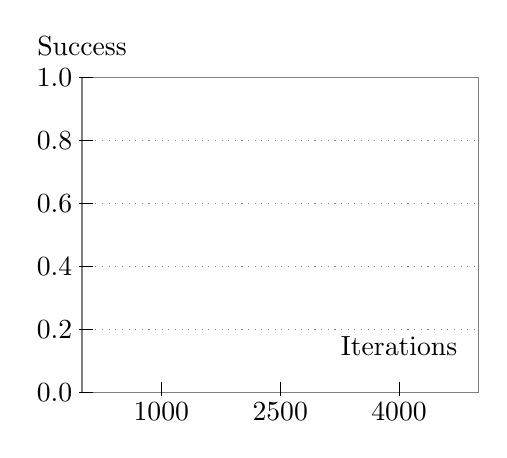
\begin{tikzpicture}[x=0.001cm,y=4cm]
    % Draw the axes and grid lines
    \draw[-,gray] (0,0) -- (0,1) -- (5000,1) -- (5000,0) -- cycle; 
    \draw[-,gray,thin, dotted, ystep=0.2, xstep=5000] (0,0) grid (5000,1);
    \foreach \x in {1000, 2500, 4000}  \draw [-,xshift=0](\x,4pt) -- (\x,-1pt);
    \foreach \y in {0.0,0.2,0.4,0.6,0.8,1.0}  \draw [-,yshift=0](4pt,\y) -- (-1pt,\y);
    \foreach \x/\xtext in {1000/1000, 2500/2500, 4000/4000} \node at (\x,0) [below] {$\xtext$};
    \foreach \y/\ytext in {0.0,0.2,0.4,0.6,0.8,1.0}  \node at (0,\y) [left] {$\ytext$};
    \node at (0,1.1) {Success};
    \node at (4000,0.15) {Iterations};
    \draw[-,gray] plot[mark=+,mark size=4,mark options={color=black}] 
			file {data/hanoid5s1r8.CP.tikzdata};
    \draw[-,gray] plot[mark=o,mark size=3,mark options={color=black}] 
			file {data/hanoid5s3r8.CP.tikzdata};
    \draw[-,gray] plot[mark=x,mark size=4,mark options={color=black}] 
			file {data/hanoid5s5r8.CP.tikzdata};

\end{tikzpicture}

}
\qquad
\subfigure[\CL+$\Omega$]{\label{fig:result-levelsB}
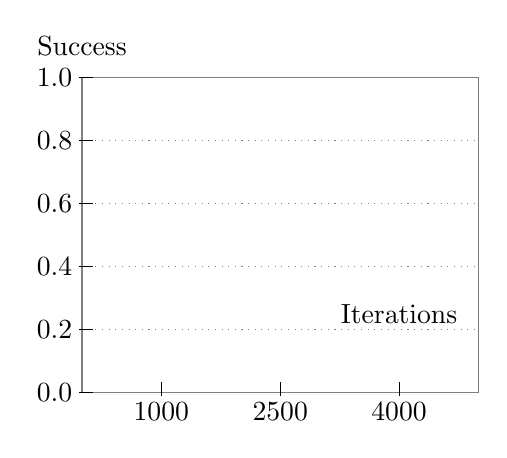
\begin{tikzpicture}[x=0.001cm,y=4cm]
    % Draw the axes and grid lines
    \draw[-,gray] (0,0) -- (0,1) -- (5000,1) -- (5000,0) -- cycle; 
    \draw[-,gray,thin, dotted, ystep=0.2, xstep=5000] (0,0) grid (5000,1);
    \foreach \x in {1000, 2500, 4000}  \draw [-,xshift=0](\x,4pt) -- (\x,-1pt);
    \foreach \y in {0.0,0.2,0.4,0.6,0.8,1.0}  \draw [-,yshift=0](4pt,\y) -- (-1pt,\y);
    \foreach \x/\xtext in {1000/1000, 2500/2500, 4000/4000} \node at (\x,0) [below] {$\xtext$};
    \foreach \y/\ytext in {0.0,0.2,0.4,0.6,0.8,1.0}  \node at (0,\y) [left] {$\ytext$};
    \node at (0,1.1) {Success};
    \node at (4000,0.25) {Iterations};
    \draw[-,gray] plot[mark=+,mark size=4,mark options={color=black}] 
			file {data/hanoid5s1r8.CF.tikzdata};
    \draw[-,gray] plot[mark=o,mark size=3,mark options={color=black}] 
			file {data/hanoid5s3r8.CF.tikzdata};
    \draw[-,gray] plot[mark=x,mark size=4,mark options={color=black}] 
			file {data/hanoid5s5r8.CF.tikzdata};

\end{tikzpicture}

}
\caption{Agent performance under \CL\ and \CL+$\Omega$ schemes for solutions at recursion levels one (pluses), three (circles) and five (crosses). Each point represents results from $5$ experiment runs using an averaging window of $100$ samples.}
\label{fig:result-levels}
\end{center}
\end{figure*}

To understand how the two approaches perform for solutions of varying difficulty we conducted a set of experiments with solutions at different recursive levels. Each experiment consisted of resolving a known set of \entity{Solve} event configurations, saved earlier as described in Section \ref{sec:setup}, whose solutions all required a given recursive depth. Figure \ref{fig:result-levels} shows that as the solution difficulty increases from one to five recursion levels, \CL\ performance drops much more significantly compared to that of \CL+$\Omega$. For instance, for solutions requiring five levels of recursion, \CL\ achieves only $50\%$ success at $5k$ iterations whereas \CL+$\Omega$ achieves $95\%$ success by $3.5k$ iterations. The poor performance of \CL\ may be attributed to the fact that deeper solutions require more \entity{move(?p2,?p)} steps and where an earlier success does not exist to guide selection at each resulting state the exploration is mostly random. On the other hand, the confidence-based measure of Equation \ref{eqn:weight} takes into account the goal-plan tree complexity and is able to guide the \CL+$\Omega$ exploration towards the deeper solutions.

Next, we conducted an experiment that consisted of resolving the full set of saved \entity{Solve} events i.e. the set contained all solutions for recursion levels one to five. Figure \ref{fig:result-fullA} shows the results for the two approaches where \CL+$\Omega$ performs better than \CL\ as expected. For the same experiment, we also recorded the number of solutions found. Figure \ref{fig:result-fullB} shows that \CL+$\Omega$ resolves all $52$ goals within $12k$ iterations whereas \CL\ resolves only $47$ by the end of the experiment at $20k$. At a similar point of comparison, to resolve $47$ goals \CL+$\Omega$ takes around $6.4k$ iterations whereas \CL\ takes more than twice as long at $17.7k$. The vertical dashed lines in Figure \ref{fig:result-fullA} and Figure \ref{fig:result-fullB} mark the $47$th and $52$nd solutions.

\begin{figure*}[t]
\begin{center}
\subfigure[Success Rate]{\label{fig:result-fullA}
../../../writeup/2010HYCAS/figs/result-fullA.tex
}
\qquad
\subfigure[Solutions Found]{\label{fig:result-fullB}
%!TEX root = ../hycas2010.tex
% Points in the input file are y-scaled by 0.5 so yval 1000 represents point 2000 in the original results. The reason for scaling was that TeX cannot handle > ~16k numbers
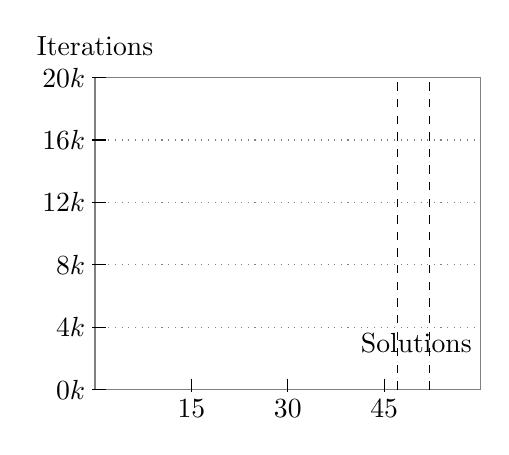
\begin{tikzpicture}[x=0.0816cm,y=.0004cm]
    % Draw the axes and grid lines
    \draw[-,gray] (0,0) -- (0,10000) -- (60,10000) -- (60,0) -- cycle; 
    \draw[-,gray,thin, dotted, ystep=2000, xstep=60] (0,0) grid (60,10000);
    \foreach \x in {15, 30, 45}  \draw [-,xshift=0](\x,4pt) -- (\x,-1pt);
    \foreach \y in {0,2000,4000,6000,8000,10000}  \draw [-,yshift=0](4pt,\y) -- (-1pt,\y);
    \foreach \x/\xtext in {15/15, 30/30, 45/45} \node at (\x,0) [below] {$\xtext$};
    \foreach \y/\ytext in {0/0k,2000/4k,4000/8k,6000/12k,8000/16k,10000/20k}  \node at (0,\y) [left] {$\ytext$};
    \node at (0,11000) {Iterations};
    \node at (50,1500) {Solutions};
    \draw[-,gray] plot[mark=o,mark size=3,mark options={color=black}] 
			file {data/hanoi5s.CP.tikzdata};
    \draw[-,gray] plot[mark=x,mark size=4,mark options={color=black}] 
			file {data/hanoi5s.CF.tikzdata};
	\draw [-,dashed](47,0pt) -- (47,10000);
	\draw [-,dashed](52,0pt) -- (52,10000);
\end{tikzpicture}

}
\caption{Agent performance under \CL\ (circles) and \CL+$\Omega$ (crosses) schemes. Each point represents an average result from $5$ experiment runs.}
\label{fig:result-full}
\end{center}
\end{figure*}

Finally, we ran a third experiment to understand the impact of applicability thresholds. In the classical BDI framework plans are either applicable or not in a boolean decision. However, in our modified framework plans are applicable according to the selection weight given by Equation \ref{eqn:weight}. Since plan execution is often not cost-free in real systems, it is likely that an adequate plan selection scheme would not select \textit{any} plan if they all have too low an expectation of success, and an agent may fail a plan without even trying. To represent this scenario we setup an applicability threshold of $20\%$ whereby plans with expectations of success less than this threshold would not be selected. In this case \CL\ shows a complete inability to learn as reported earlier \cite{Singh:AAMAS10}. In contrast \CL+$\Omega$ benefits from the adjusted selection weights of Equation \ref{eqn:weight} and shows similar performance as before (Figure \ref{fig:result-fullA})\footnote{The threshold of $0.2$ while somewhat arbitrary is consistent with that used earlier \cite{Singh:AAMAS10}. The difference between the default weight ($0.5$) and the threshold weight ($0.2$ in this case) decides how much ``give'' we have in the exploration. The closer the threshold is to $0.5$ the greater the chance that the plan will be aborted before a solution is found.}.

%A final observation in Figure \ref{fig:result-full} is that neither approach converges to $1.0$. This is because the Hanoi domain is not free from goal inter-dependence. So if a plan learns to solve a sub-goal in two ways that each lead to different end states, then depending on the way the sub-goal was resolved the top level goal may pass or fail. Indeed, when we analyse the result log we find that \CL+$\Omega$ finds all solutions as expected, but even so fails now and then for some of these because of the way a sub-goal was realised. Our learning framework does not currently support goal inter-dependence.

A final observation in Figure \ref{fig:result-fullA} is that \CL+$\Omega$ does not reach the performance of the hand-crafted JACK program and converges to about $90\%$ success even though it successfully discovers all solutions.
This is because the decision tree representation does not guarantee that the training data will always be correctly classified (we discuss this accuracy versus compactness trade-off in Section \ref{sec:decision_trees}). For instance, a decision tree may report a poor likelihood of success for a given state even when the associated training sample indicates success, due to the sample being misclassified in the failure ``class''. The only way to guarantee correctness would be to use the training data directly, for instance using a look-up table. Furthermore, when the learnt decision trees are converted to rules they do not ``look'' like the original ones but are far more complex. This is mainly due to representational differences as our simple representation is propositional whereas the original conditions are relational.
